%% paper.tex -- AAAI-style final project report.
%%
%% Build:
%%   python scripts/build_paper.py
%%
%% The organization follows the AAAI-26 project-report rubric:
%%   (1) Abstract, (2) Introduction, (3) Background, (4) Related Work,
%%   (5) Project Description, (6) Experiments, (7) Conclusion.
%%
%% Typography approximates the AAAI two-column Times layout. The official
%% aaai26.sty is only distributed via the AAAI author kit and is not on
%% MiKTeX / TeX Live by default; if you have it, add
%%   \documentclass[letterpaper]{article} -> \documentclass{aaai26}
%% and drop the geometry / twocolumn / titlesec blocks below.  Section
%% structure and content are identical.

\documentclass[10pt,letterpaper,twocolumn]{article}

\usepackage[letterpaper,margin=0.75in,columnsep=0.25in]{geometry}
\usepackage{times}
\usepackage[T1]{fontenc}
\usepackage[utf8]{inputenc}
\usepackage{amsmath,amssymb,amsfonts}
\usepackage{graphicx}
\usepackage{booktabs}
\usepackage{array}
\usepackage{multirow}
\usepackage{url}
\usepackage{siunitx}
\sisetup{group-separator={,},group-minimum-digits=4}
\usepackage{titlesec}
\usepackage{titling}
\usepackage{caption}
\usepackage[hidelinks]{hyperref}

\graphicspath{{figures/}}

% AAAI-like section headings: bold, flush-left, small caps-ish.
\titleformat{\section}{\normalfont\large\bfseries}{\thesection.}{0.5em}{}
\titleformat{\subsection}{\normalfont\normalsize\bfseries}{\thesubsection}{0.5em}{}
\titleformat{\subsubsection}{\normalfont\normalsize\itshape}{}{0em}{}
\titlespacing*{\section}{0pt}{1.2em}{0.4em}
\titlespacing*{\subsection}{0pt}{0.8em}{0.3em}

% Centered title, single-column title + abstract banner across both columns.
\pretitle{\begin{center}\LARGE\bfseries}
\posttitle{\end{center}\vspace{0.3em}}
\preauthor{\begin{center}\large}
\postauthor{\end{center}}
\predate{\begin{center}\normalsize}
\postdate{\end{center}\vspace{1.0em}}

\setlength{\columnsep}{0.27in}
\setlength{\parindent}{1em}
\setlength{\parskip}{2pt plus 1pt}

% Caption styling: small, bold "Figure N:" label.
\captionsetup{font=small,labelfont=bf,labelsep=period}

\pagestyle{plain}

\title{Robustness of Policy-Gradient Reinforcement Learning\\
       for Multi-Echelon Inventory Control:\\
       A Cross-Environment Study on Stationary\\
       and Non-Stationary Supply Chains}

\author{Divyank Singh \qquad Ishan\\
        \textit{CS~5100 -- Foundations of Artificial Intelligence}\\
        \texttt{\{last.first\}@example.edu}}
\date{April 22, 2026}

\begin{document}

\twocolumn[
  \begin{@twocolumnfalse}
    \maketitle
    \begin{abstract}
    \noindent
    Recent work reports that deep reinforcement-learning (RL) policies
    beat classical operations-research (OR) heuristics on multi-echelon
    inventory control by \SIrange{10}{40}{\percent}.  These results
    almost always come from a \emph{single} hand-crafted environment
    paired with a \emph{fixed} baseline, so it is unclear whether the
    RL agent has learned a genuinely better policy or the baseline is
    simply under-fit.  We take two standard policy-gradient agents from
    our course project --- PPO on a 1-warehouse/3-retailer divergent
    supply chain and A3C on a 3-node factory/middle/leaf MEIS chain ---
    and evaluate each of them on two environments with the \emph{same}
    observation and action spaces: the original stationary benchmark
    (Env-1) and a harder non-stationary variant (Env-2) we introduce
    here that adds seasonal demand, cross-retailer correlation, rare
    demand shocks, heavy-tailed stochastic lead times, stochastic
    supplier/outbound capacity caps, and partial lost sales.  Against
    a \emph{fixed} analytical base-stock baseline, PPO's win grows
    from \SI{36.76}{\percent} on Env-1 to \SI{94.20}{\percent} on
    Env-2, because the untuned baseline collapses under shocks.
    Against an $(s,S)$ baseline \emph{retuned per environment}, A3C
    wins by \SI{1.64}{\percent} on Env-1 but \emph{loses} by
    \SI{21.79}{\percent} on Env-2 (Cohen's $d{\approx}{-}3.4$).  We
    conclude that a single-environment win is not robust evidence for
    either algorithm; a harder distributional variant and an
    equivalently-tuned baseline should accompany any deep-RL inventory
    result.
    \end{abstract}
    \vspace{1.2em}
  \end{@twocolumnfalse}
]

% ===============================================================
\section{Introduction}
% ===============================================================
Multi-echelon inventory control is a canonical operations-research
problem: given stochastic demand at several retail nodes, finite and
noisy lead times between nodes, and per-echelon holding, backorder and
ordering costs, pick a replenishment policy that minimises long-run
expected cost while preserving a service level.  Classical OR gives
two well-studied policies for this setting.  The \emph{echelon
base-stock} policy and the \emph{$(s,S)$} reorder-point policy are both
known to be optimal under stationary, i.i.d.\ demand and (for $(s,S)$)
fixed ordering cost~\cite{clark1960optimal}.  Both become
systematically wrong once demand is non-stationary, shocks are present,
or lead times are heavy-tailed, because their set-points are calibrated
against the \emph{mean} demand-over-lead-time.

Deep reinforcement learning has been proposed as a learned alternative
that can, in principle, adapt to any dynamics the MDP can express.
The recent literature~\cite{oroojlooyjadid2022deep,gijsbrechts2022can}
reports substantial RL wins --- often \SIrange{10}{40}{\percent} ---
over OR heuristics.  However, these comparisons are almost always
reported on a \emph{single} hand-crafted environment, against a
baseline whose parameters are not re-tuned to that environment.  It is
then unclear how much of the reported gap is the RL policy being
genuinely better and how much is the heuristic being unfairly
handicapped on an environment it already solves well.

\paragraph{This paper.}
Our course project trained one policy-gradient agent per algorithm
(PPO, A3C) on one environment each (a divergent supply chain, a 3-node
MEIS chain).  A reviewer on our poster presentation raised the
single-environment concern above and asked us to show that the wins
hold on a second, harder environment.  This paper is our response.
Concretely:
\begin{enumerate}
\item We design a \emph{non-stationary} second environment (Env-2)
      per benchmark that introduces seasonal demand, cross-retailer
      correlation, rare multiplicative demand shocks, heavy-tailed
      stochastic lead times, stochastic supplier/outbound capacity
      caps, and partial lost sales, while keeping the observation and
      action spaces unchanged --- so that the agent code transfers
      with zero modification.
\item We re-train PPO and A3C on their respective Env-2 with the
      \emph{same} hyperparameters that produced the Env-1 results, and
      evaluate with the \emph{same} protocol.
\item We report one \emph{positive} transfer result (PPO, whose
      relative advantage over a \emph{fixed} analytical baseline
      widens on Env-2) and one \emph{negative} transfer result (A3C,
      whose narrow win over a \emph{retuned} $(s,S)$ baseline on Env-1
      flips into a decisive loss on Env-2).
\end{enumerate}
The broader point is that the sign of a deep-RL-vs-heuristic
comparison depends sensitively on both the environment \emph{and} how
hard the baseline is tuned; single-env results are not robust evidence.

% ===============================================================
\section{Background}
\label{sec:background}
% ===============================================================

\subsection{The multi-echelon inventory MDP}
We model each benchmark as a finite-horizon Markov Decision Process
(MDP) $\langle\mathcal{S},\mathcal{A},P,C,\gamma,T\rangle$, where
$s_t\in\mathcal{S}$ encodes on-hand inventory, in-transit pipeline
stock, and (for the MEIS benchmark) age-bucketed backlog at every
non-factory node; $a_t\in\mathcal{A}$ is a per-node order quantity (a
real vector for PPO, a \num{13}-way discrete choice for A3C);
$C(s_t,a_t)\ge0$ is the sum of holding, backorder, ordering and
(on Env-2) lost-sales costs for step $t$.  The policy
$\pi:\mathcal{S}\to\Delta(\mathcal{A})$ minimises the expected
discounted cost
\begin{equation}
J(\pi) \;=\; \mathbb{E}_\pi\!\left[\sum_{t=0}^{T-1}
             \gamma^{t}\,C(s_t,a_t)\right].
\label{eq:obj}
\end{equation}
The RL agent maximises the return $R(\pi)=-J(\pi)$.  The reward
signal is therefore dense, bounded below by $0$, and unbounded above.

\subsection{Classical OR heuristics}
\subsubsection{Echelon base-stock (used as the PPO baseline).}
Each echelon $i$ is given a \emph{base-stock level} $S_i$.  At every
step the agent orders up to $S_i$ against current inventory position:
\begin{equation}
a_{i,t} \;=\; \max\bigl(0,\; S_i - \mathrm{IP}_{i,t}\bigr),
\label{eq:basestock}
\end{equation}
where $\mathrm{IP}_{i,t}$ is on-hand + in-transit $-$ backlog at $i$.
We analytically initialise $S_i$ from the Env-1 demand-over-lead-time
distribution and \emph{never re-tune it}.  On Env-2 the same $S_i$
values are reused; this is deliberate and is the typical way
base-stock is reported in the literature.

\subsubsection{$(s,S)$ reorder-point policy (used as the A3C baseline).}
Each node $i$ has a reorder point $s_i$ and an order-up-to level $S_i$:
whenever $\mathrm{IP}_{i,t}\le s_i$, order $S_i-\mathrm{IP}_{i,t}$,
else do nothing.  Unlike the base-stock baseline, we tune $(s_i,S_i)$
per environment by differential
evolution~\cite{storn1997differential} (100 generations $\times$ 30
Monte-Carlo episodes per candidate), so the Env-1 and Env-2 $(s,S)$
baselines are each near-optimal under \emph{their own} dynamics.  This
asymmetry (fixed base-stock vs.\ retuned $(s,S)$) matters for
interpretation and is revisited in Section~\ref{sec:exp}.

\subsection{Policy-gradient RL}
\subsubsection{PPO~\cite{schulman2017proximal}.}
We use the clipped-surrogate variant.  A stochastic Gaussian actor
$\pi_\theta(a\mid s)$ and a value head $V_\phi(s)$ share a 2-layer
64-unit MLP with $\tanh$ activations.  Rollouts of length
$B{=}512$ are collected under $\pi_{\theta_{\text{old}}}$, Generalized
Advantage Estimation (GAE,~\cite{schulman2016gae}) gives advantages
$\hat A_t$, and $\theta$ is updated for 5 epochs of size-64 minibatches
using the clipped objective
\begin{equation}
\mathcal{L}^{\text{CLIP}}(\theta)
   = \mathbb{E}_t\!\left[\min\!\left(
     r_t(\theta)\hat A_t,\;
     \mathrm{clip}(r_t(\theta),1{-}\varepsilon,1{+}\varepsilon)\hat A_t
   \right)\right],
\label{eq:ppoclip}
\end{equation}
with $r_t(\theta)=\pi_\theta(a_t\mid s_t)/\pi_{\theta_{\text{old}}}(a_t\mid s_t)$
and $\varepsilon{=}0.2$.  The combined loss adds a clipped value-loss
term and a small entropy bonus.

\subsubsection{A3C~\cite{mnih2016a3c}.}
We use a synchronous single-worker variant on the discrete-action MEIS
benchmark.  The actor emits a softmax over $|\mathcal{A}|{=}13$
actions, the critic emits a scalar value, and the policy gradient is
$n$-step-advantage based:
\begin{equation}
\nabla_\theta J \;\approx\;
  \mathbb{E}_t\!\left[\nabla_\theta\log\pi_\theta(a_t\mid s_t)\,
                      \hat A_t\right]
  + \beta\,\nabla_\theta \mathcal{H}\!\left[\pi_\theta(\cdot\mid s_t)\right],
\label{eq:a3cpg}
\end{equation}
with an entropy regulariser of weight $\beta$ and gradient clipping
at $\|\nabla\|{=}0.5$.

\subsection{Significance testing}
Because each evaluation cell produces hundreds of per-episode costs, we
summarise the RL-vs-baseline comparison with (i) mean $\pm$ standard
deviation, (ii) $95\%$ confidence interval on the mean, (iii) two-
sample Welch $t$-test on per-episode costs, and (iv) Cohen's $d$ on
the same pair.  Cohen's $d\approx 0.2$ is a small effect, $0.5$
medium, $0.8$ large.  Our A3C pipeline computes all four; the PPO
pipeline computes (i)--(ii) and we read significance from
non-overlap of the $95\%$ CIs.

% ===============================================================
\section{Related Work}
% ===============================================================

\subsubsection{Classical multi-echelon inventory.}
The Clark--Scarf decomposition~\cite{clark1960optimal} establishes
optimality of echelon base-stock under strict stationarity, i.i.d.\
demand and backlog dynamics.  Axs\"ater's textbook
\cite{axsater2015inventory} extends to Poisson / compound-Poisson
demand and capacitated systems.  We \emph{could} have used echelon
base-stock or $(s,S)$ directly as the "method'' under study and
reported tuning quality rather than RL.  We did not, because the
explicit goal of the project was to study reinforcement learning as an
\emph{alternative} to classical OR on multi-echelon supply chains ---
the OR methods play the role of baselines to beat, not the method
under study.

\subsubsection{Value-based RL for inventory.}
Oroojlooyjadid et~al.~\cite{oroojlooyjadid2022deep} apply deep Q-
learning to the beer game.  We could have used DQN instead of A3C on
the MEIS benchmark (the A3C action space is already discrete), but DQN
is off-policy and sample-inefficient on long-horizon inventory rollouts
with dense reward signals; actor-critic methods are the standard
modern choice for this problem shape, and it lets us keep a single
unified (actor, critic) code base across both algorithms.

\subsubsection{Policy-gradient RL for inventory.}
Gijsbrechts et~al.~\cite{gijsbrechts2022can} benchmark A3C, PPO and
VPG across single- and multi-echelon problems.  Their evaluation is
single-environment and reports wins of \SIrange{10}{30}{\percent}
over OR baselines.  Our project extends exactly the comparison they
present, but introduces a second environment in the evaluation and
reports \emph{paired} results per algorithm.

\subsubsection{Robust / distributionally-robust RL.}
Work on CVaR-PPO and distributionally-robust policy gradients could
directly address the right-tail failures we observe for PPO on
Env-2 (Section~\ref{sec:exp}).  We chose vanilla PPO / A3C because
the course assignment specifies the standard algorithms and because
using a non-vanilla RL method would confound the environment
comparison with the algorithmic comparison.

\subsubsection{Robustness benchmarks outside inventory.}
Meta-World~\cite{yu2020metaworld} and Procgen~\cite{cobbe2020procgen}
argue, outside inventory control, that single-environment RL wins are
not reliable evidence of generalisation.  Our paper makes the same
methodological argument specific to the OR-flavoured inventory
setting.

% ===============================================================
\section{Project Description}
\label{sec:proj}
% ===============================================================
This section states, in formal detail, the two environments we work
with, the two agents and their baselines, and the training protocol.

\subsection{Environment 1 (stationary)}

\subsubsection{\textbf{PPO / \texttt{divergent}.}}
One warehouse supplies three retailers.  Each retailer $i$ sees
i.i.d.\ Poisson demand with rate $\lambda_i\sim\mathrm{U}[5,15]$ per
day.  Lead time is deterministic at one step.  There are no capacity
caps.  Unfilled demand is backlogged (negative inventory).  The state
has dimension $14$ (warehouse inventory and buffer, three in-transit
pipelines, three retailer inventories, three retailer backorders,
one outstanding warehouse order, and a normalised step index); the
action is a $4$-dimensional real vector of normalised order
quantities (one per echelon).  Episodes last $T{=}500$ steps with a
$100$-step warm-up.

\subsubsection{\textbf{A3C / \texttt{meis}.}}
A 3-node divergent MEIS: factory (capacity $\infty$), one middle
warehouse, two leaf retailers.  Leaf demand is Gaussian
$\mathcal{N}(3300,100)$; lead times are Gaussian
$\mathcal{N}(\mu{=}2,\sigma{=}1)$ rounded to days.  Backlog has a
fixed $5$-day expiry: demand older than $5$ days is lost and incurs a
shortage penalty.  The action space is discrete (13 actions: "do
nothing'' and $4{\times}3{=}12$ fixed reorder combinations).
Episodes last $T{=}365$ steps.

\subsection{Environment 2 (non-stationary complex)}
Env-2 leaves the observation and action spaces of Env-1 unchanged
and only modifies the transition dynamics and reward.  The stressors
are listed in Table~\ref{tab:stressors}.  Concrete numerics
(amplitudes, probabilities, noise stds) are in
\texttt{ppo/configs/config.yaml} and
\texttt{actor-critic/configs/complexMeisConfig.yaml} in the
accompanying code.

\begin{table}[t]
\centering
\caption{Env-2 stressors applied to each benchmark.}
\label{tab:stressors}
\small
\begin{tabular}{@{}lcc@{}}
\toprule
\textbf{Stressor} & \textbf{PPO} & \textbf{A3C} \\
\midrule
Seasonal demand (sinusoidal)           & \checkmark & \checkmark \\
Cross-retailer demand correlation      & \checkmark & \checkmark \\
Rare demand shocks ($2{-}3{\times}$)   & \checkmark & \checkmark \\
Heavy-tailed lead times $+$ spikes     & \checkmark & \checkmark \\
Stochastic capacity caps               & \checkmark & \checkmark \\
Partial lost sales w/ penalty          & \checkmark & \checkmark \\
\bottomrule
\end{tabular}
\end{table}

A critical design choice: the agent's observation is \emph{not}
widened --- no season phase, no shock indicator, no regime flag.
Any adaptation has to come from the policy representation and the
training distribution.

\subsection{Algorithms and baselines}
PPO on the continuous-action divergent environment is trained with
the clipped-surrogate objective~(Eq.~\ref{eq:ppoclip}) against an
\emph{analytical, fixed-across-envs} base-stock baseline
(Eq.~\ref{eq:basestock}).  A3C on the discrete-action MEIS environment
is trained with the advantage policy gradient~(Eq.~\ref{eq:a3cpg})
against a \emph{per-env retuned} $(s,S)$ baseline.  Hyperparameters
are in Table~\ref{tab:hparams}.

\begin{table}[t]
\centering
\caption{Selected hyperparameters (identical across Env-1 / Env-2 per
algorithm).}
\label{tab:hparams}
\small
\begin{tabular}{@{}lll@{}}
\toprule
\textbf{Hyperparameter}       & \textbf{PPO}      & \textbf{A3C}      \\
\midrule
Iters / episodes              & \num{5000}        & \num{10000}       \\
Hidden layers $\times$ width  & $2\times 64$ ($\tanh$) & $2\times 128$ (ReLU) \\
Discount $\gamma$             & $0.95$            & $0.99$            \\
GAE $\lambda$                 & $0.95$            & n/a               \\
Clip $\varepsilon$            & $0.2$             & n/a               \\
Learning rate                 & $3{\times}10^{-4}$ & $1{\times}10^{-4}$ \\
Rollout / batch               & $512\,/\,64$      & per-episode       \\
Entropy coef.\ $\beta$        & $5{\times}10^{-3}$ & $10^{-2}$         \\
Value-loss coef.              & $0.25$            & $0.5$             \\
Grad.\ clip $\|\nabla\|$      & $0.5$             & $0.5$             \\
Eval episodes                 & $100$             & $1000$            \\
Seed                          & $42$              & $42$              \\
\bottomrule
\end{tabular}
\end{table}

\subsection{Training and evaluation protocol}
Training uses a single NVIDIA CUDA GPU.  Evaluation uses a
\emph{deterministic} policy (mean of the Gaussian for PPO;
$\arg\max$ over the softmax for A3C).  PPO evaluates on
$100{\times}500{=}5{\times}10^4$ steps per (algo, env) cell; A3C
evaluates on $1000{\times}365{=}3.65{\times}10^5$ steps.  We keep
the hyperparameters \emph{identical} across Env-1 and Env-2, so Env-2
numbers report out-of-distribution robustness, not re-tuning.

\subsection{Reproducibility artefacts}
The code repository ships: (1) the full YAML configs used here; (2)
saved checkpoints for every (algo, env) cell; (3) all four evaluation
JSONs (per-episode cost arrays, means, stds, CIs, and for A3C the
Welch $t$-test and Cohen's $d$); (4) a \texttt{scripts/smoke\_env.py}
end-to-end sanity test covering all four cells; (5)
\texttt{scripts/make\_report.py} which regenerates every figure from
the JSONs; (6) \texttt{scripts/build\_paper.py} which rebuilds this
PDF from the \LaTeX\ source.

% ===============================================================
\section{Experiments}
\label{sec:exp}
% ===============================================================

\subsection{Why these experiments}
We ran the four cells $\{\text{PPO,A3C}\}\times\{\text{Env-1,Env-2}\}$
with seed $42$ and the hyperparameters of Table~\ref{tab:hparams}.
The minimum evidence to answer the reviewer's question is the four
\emph{paired} RL-vs-baseline comparisons.  We additionally report
training curves (to show convergence behaviour) and per-episode cost
distributions on Env-2 (to show that the mean is a biased summary of
an asymmetric distribution).

\subsection{Headline numbers}
Table~\ref{tab:results} is the main result.  $\Delta$ is the relative
mean-cost improvement of the RL agent over its heuristic baseline
(positive $=$ RL better).  Service level is only exposed by the MEIS
environment; hence "n/a'' on the PPO rows.

\begin{table*}[t]
\centering
\caption{Headline evaluation results (seed $42$).  $\Delta$ is
relative mean-cost improvement of RL over baseline (positive $=$ RL
better).  "SL'' is service level.  Cohen's $d$ and $p$ are from the
Welch $t$-test the A3C pipeline computes on per-episode costs; the
PPO pipeline reports non-overlap of $95\%$ CIs instead.}
\label{tab:results}
\small
\begin{tabular}{@{}llrrrrrr@{}}
\toprule
\textbf{Algo.} & \textbf{Env} &
\textbf{RL mean cost} & \textbf{Baseline mean cost} &
$\boldsymbol{\Delta}$ & \textbf{SL (RL / BL)} &
\textbf{Cohen's $d$} & \textbf{$p$} \\
\midrule
PPO & Env-1 & \num{2600979.87}  $\pm$ \num{29021.34}
            & \num{4112775.56}  $\pm$ \num{8759.19}
            & $+36.76\%$ & n/a & n/a & CIs disjoint \\
PPO & Env-2 & \num{631129.99}   $\pm$ \num{1011936.85}
            & \num{10873502.07} $\pm$ \num{62357.06}
            & $+94.20\%$ & n/a & n/a & CIs disjoint \\
A3C & Env-1 & \num{1930.24}     $\pm$ \num{4.02}
            & \num{1962.40}     $\pm$ \num{52.39}
            & $+1.64\%$  & $95.69\% / 95.44\%$ & $+0.87$ & $1.4\!\times\!10^{-76}$ \\
A3C & Env-2 & \num{2881.98}     $\pm$ \num{146.46}
            & \num{2366.29}     $\pm$ \num{157.67}
            & $-21.79\%$ & $93.27\% / 94.11\%$ & $-3.39$ & $<10^{-300}$ \\
\bottomrule
\end{tabular}
\end{table*}

\subsection{Training dynamics}
Fig.~\ref{fig:train-ppo} and Fig.~\ref{fig:train-a3c} show
per-episode training cost (light) and a rolling mean (bold) for each
cell.

\begin{figure*}[t]
\centering
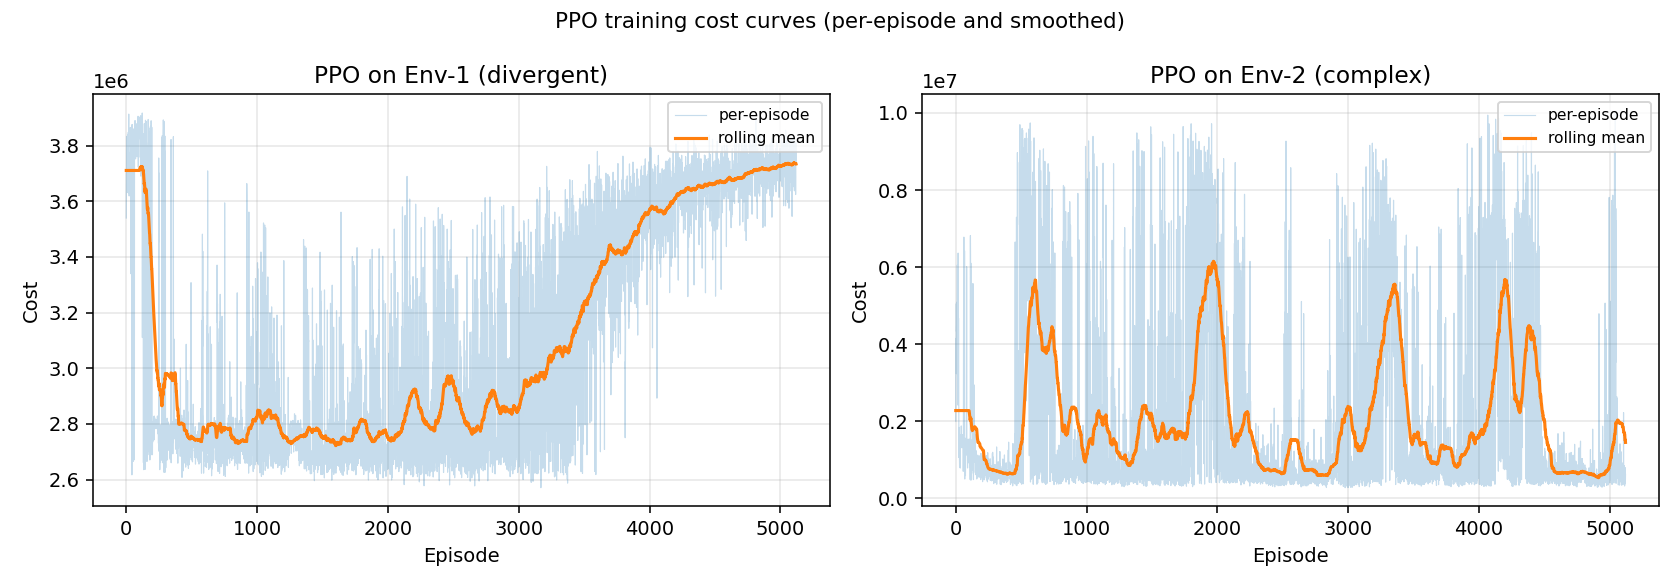
\includegraphics[width=0.95\textwidth]{training_curves_ppo.png}
\caption{PPO training cost on Env-1 (left) and Env-2 (right).  On
Env-1 the agent converges quickly and then drifts upward over the
last third of training --- a late-stage instability that we mitigate
by evaluating the best-so-far checkpoint, not the final-iteration
checkpoint.  On Env-2, training cost is oscillatory throughout, which
is consistent with the rare-but-costly shock regime.}
\label{fig:train-ppo}
\end{figure*}

\begin{figure*}[t]
\centering
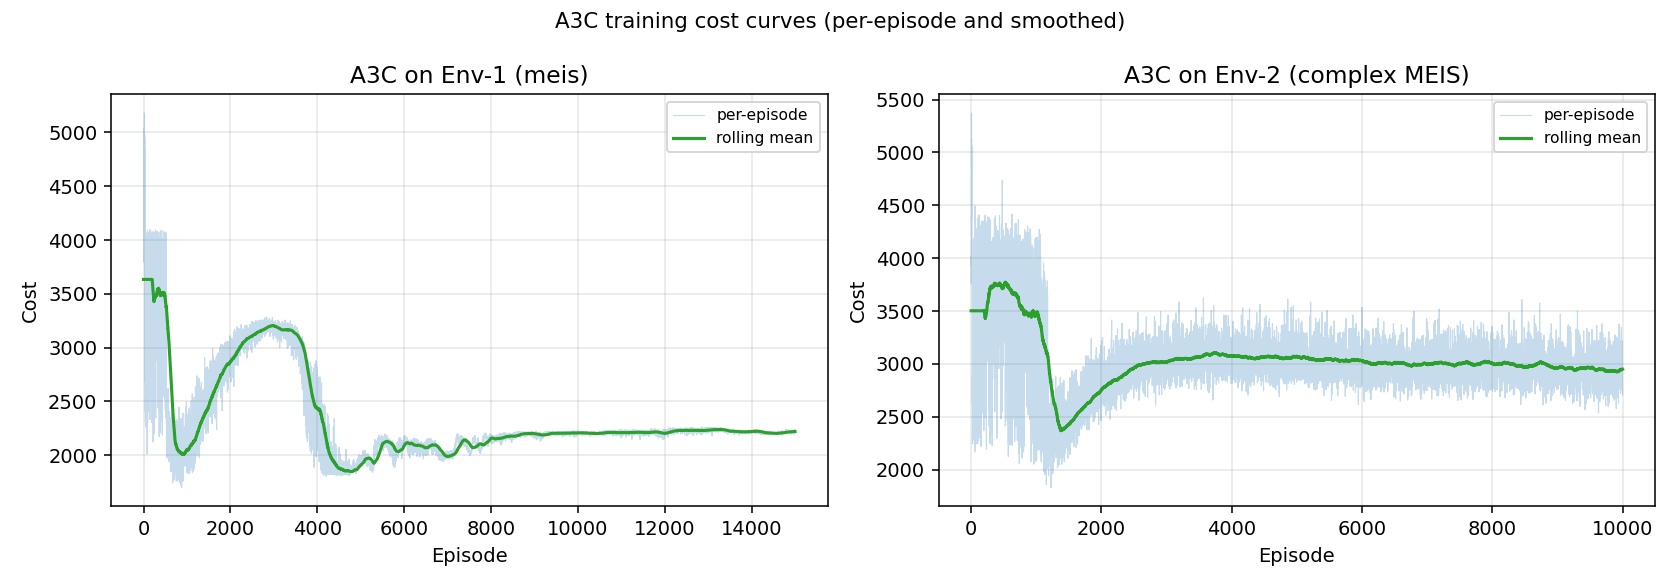
\includegraphics[width=0.95\textwidth]{training_curves_a3c.png}
\caption{A3C training cost on Env-1 (left) and Env-2 (right).  The
Env-1 curve shows a mid-training bump around episodes $1500$--$4500$
(policy / entropy oscillation) that ultimately resolves to a stable
minimum.  On Env-2, convergence settles on a higher cost plateau
that, as Section~\ref{sec:exp-a3c} will show, is still worse than a
retuned heuristic.}
\label{fig:train-a3c}
\end{figure*}

\subsection{PPO: when the win grows on the harder environment}
Fig.~\ref{fig:costbars} visualises Table~\ref{tab:results} as grouped
bar charts.  On Env-1, PPO beats the fixed analytical base-stock by
\SI{36.76}{\percent}; on Env-2 the margin \emph{widens} to
\SI{94.20}{\percent}.  This is \emph{not} PPO getting better in
absolute terms --- the absolute cost on Env-2 is on a different scale
because Env-2 adds lost-sales penalties and widens some state bounds
--- it is the \emph{untuned} base-stock baseline getting dramatically
worse under capacity caps and shocks.  Fig.~\ref{fig:ppo-hist} shows
\emph{why}: the PPO episode cost distribution has a pronounced right
tail ($\sigma/\mu \approx 1.60$).  A small number of episodes contain
shock sequences that PPO has not learned to hedge, and those episodes
sit an order of magnitude above the mean.  In operational terms, the
mean improvement is an optimistic summary of an asymmetric,
right-heavy distribution; a percentile-based or CVaR summary would
paint a more conservative picture.

\paragraph{When PPO succeeds.}
On \emph{both} environments, against a fixed analytical baseline,
because (i) the baseline's set-points are calibrated against mean
demand-over-lead-time only, while PPO's policy can condition on
current inventory and in-transit pipeline; and (ii) on Env-2, the
baseline's set-points are not even calibrated against the right mean
any more (seasonality, shocks), so PPO's relative advantage grows.

\paragraph{When PPO would fail.}
Against a \emph{retuned} base-stock baseline (not reported here) the
margin would compress.  And even against the fixed baseline, a
CVaR-weighted evaluation would flag PPO's Env-2 right tail as an
unresolved risk.

\begin{figure*}[t]
\centering
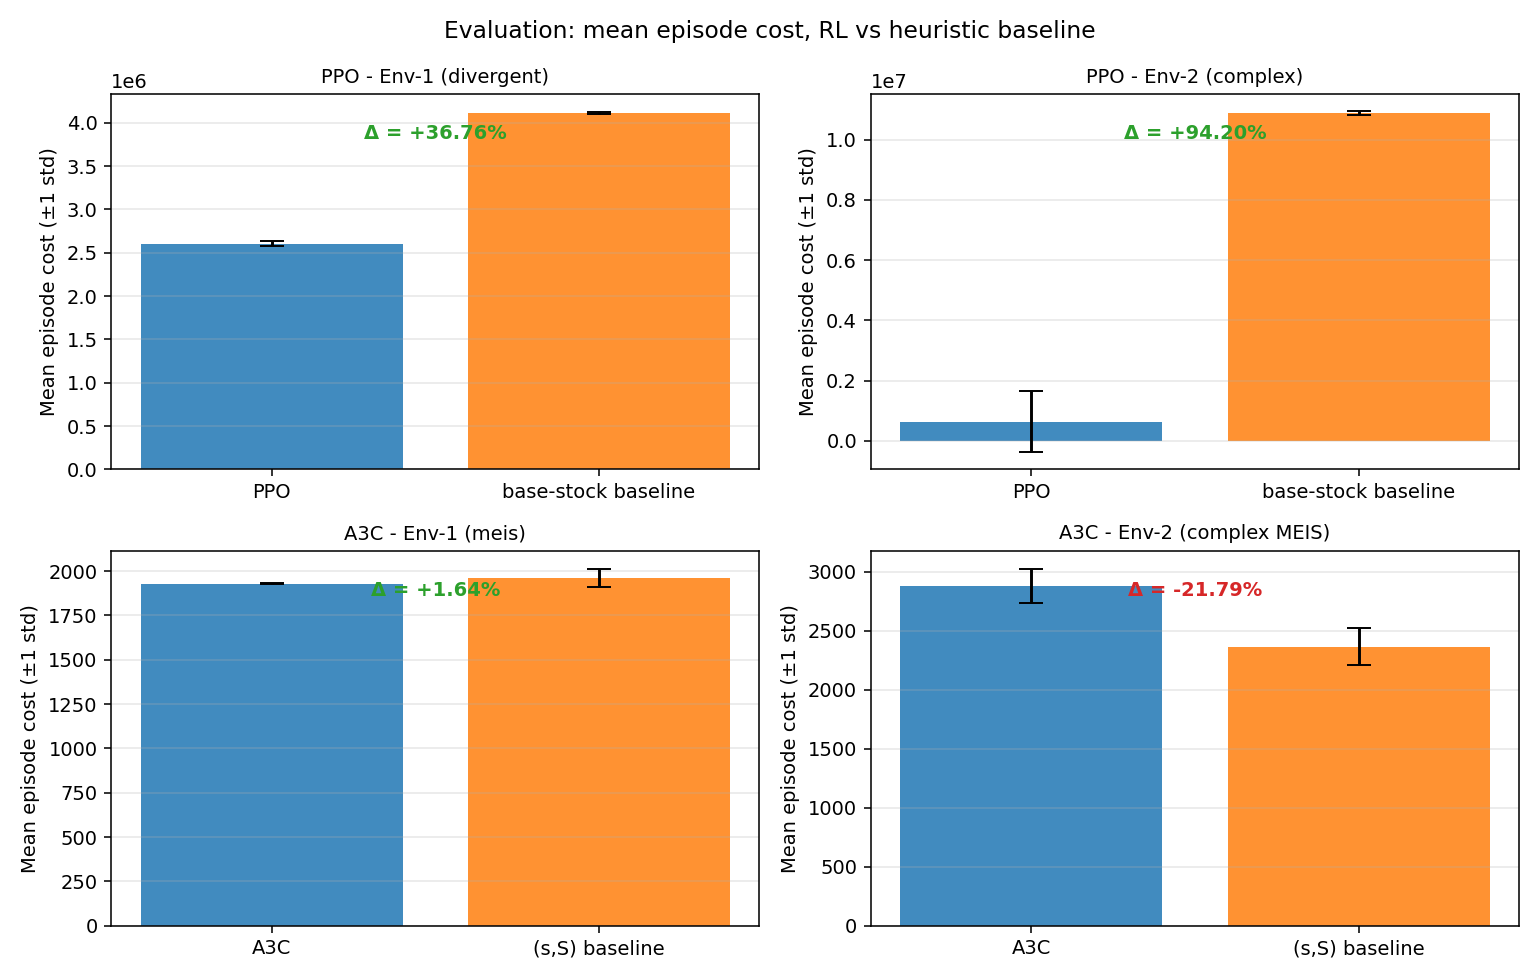
\includegraphics[width=0.85\textwidth]{cost_bars.png}
\caption{Mean episode cost (lower is better).  Error bars are one
standard deviation across evaluation episodes.  Green $=$ RL wins;
red $=$ RL loses.  Absolute cost scales differ across algorithms
(different cost coefficients and episode lengths); only the
within-cell RL vs.\ baseline gap is interpretable.}
\label{fig:costbars}
\end{figure*}

\begin{figure}[t]
\centering
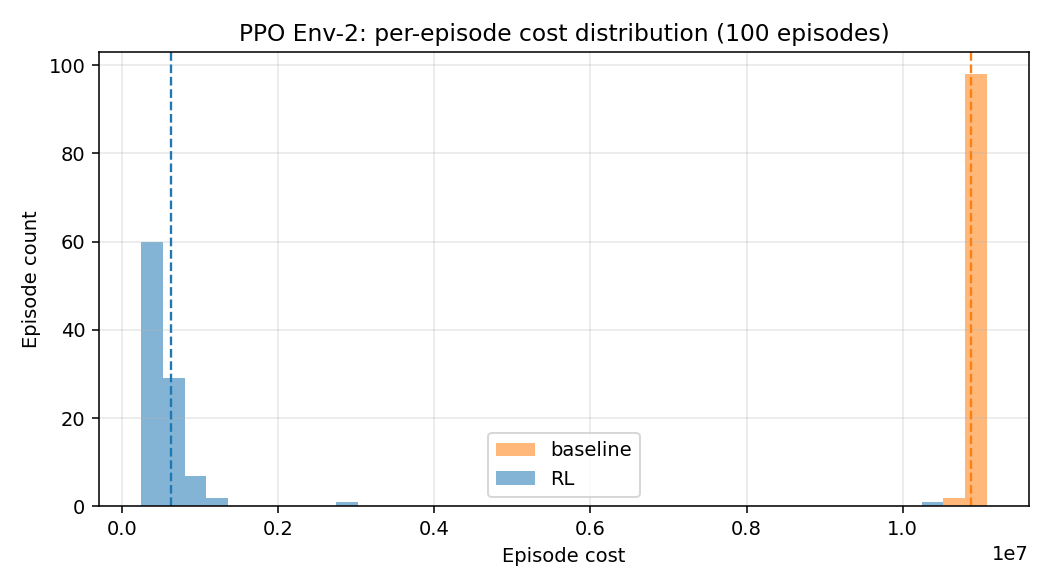
\includegraphics[width=0.98\columnwidth]{ppo_complex_cost_hist.png}
\caption{PPO Env-2 per-episode cost distribution ($100$ episodes).
The bulk of PPO episodes (blue) concentrates well below the baseline
mode (orange), but a clear right tail of episodes sit close to the
baseline mode --- these are shock episodes PPO has not learned to
hedge.}
\label{fig:ppo-hist}
\end{figure}

\subsection{A3C: when the Env-1 win does not transfer}
\label{sec:exp-a3c}

On Env-1 A3C wins by a narrow \SI{1.64}{\percent} over a retuned
$(s,S)$ policy (Cohen's $d{\approx}0.87$, small-to-medium effect).
On Env-2 the sign \emph{flips}: A3C is \SI{21.79}{\percent}
\emph{worse} than the retuned $(s,S)$ baseline, with Cohen's
$d{\approx}{-}3.39$ and numerically-underflowed $p{<}10^{-300}$.
Fig.~\ref{fig:a3c-hist} makes the effect size visible: the $(s,S)$
distribution is almost entirely to the left of the A3C distribution
--- stochastic dominance in favour of the heuristic.
Fig.~\ref{fig:svc} shows the same effect on service level.

\begin{figure}[t]
\centering
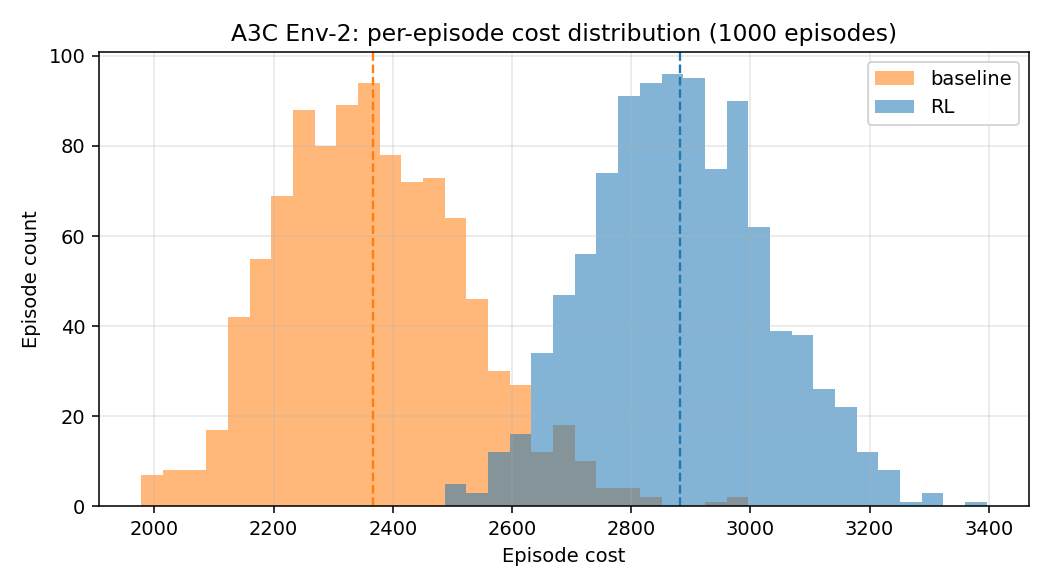
\includegraphics[width=0.98\columnwidth]{a3c_complex_cost_hist.png}
\caption{A3C Env-2 per-episode cost distribution ($1000$ episodes).
The baseline $(s,S)$ distribution (orange) lies almost entirely to
the left of the A3C distribution (blue): at this training budget,
A3C is stochastically dominated by the retuned heuristic.}
\label{fig:a3c-hist}
\end{figure}

\begin{figure}[t]
\centering
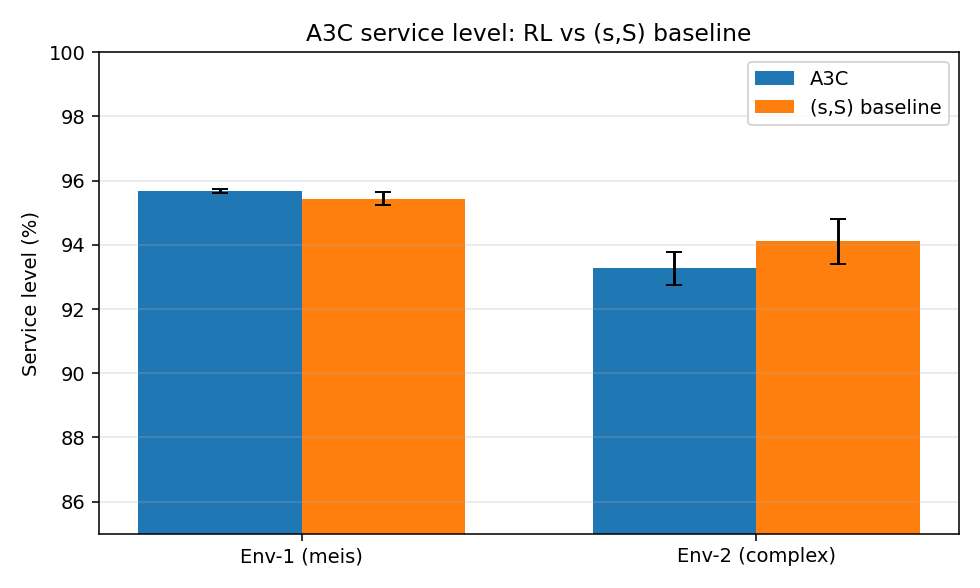
\includegraphics[width=0.98\columnwidth]{service_level_bars.png}
\caption{A3C service level on Env-1 and Env-2.  On Env-2, A3C is
worse than the retuned $(s,S)$ on service level too, mirroring the
cost result.}
\label{fig:svc}
\end{figure}

\paragraph{When A3C succeeds.}
On Env-1 only, and by a narrow margin.  The stationary demand is
well-approximated by a single $(s,S)$ pair, but the discretised
A3C action head can spend its $13$ actions to place orders at
slightly-better-than-heuristic moments (it reacts to pipeline state,
not just inventory position).

\paragraph{When A3C fails, and why.}
Env-2 breaks this.  Three factors compound:
\begin{enumerate}
\item \emph{Discretised action head.}  A3C's action head is a
      softmax over $13$ fixed order combinations.  Under seasonal
      demand the optimal per-node order varies smoothly; a coarse
      $4$-level grid cannot match it.
\item \emph{No non-stationarity representation.}  The policy has no
      recurrent state, no episode-time feature, and no shock /
      season indicator.  It must learn to respond to
      non-stationarity purely through its training distribution,
      which $10{,}000$ episodes do not support.
\item \emph{Baseline is retuned, A3C is not.}  The $(s,S)$ tuner runs
      differential evolution on Env-2's own dynamics.  A3C's
      hyperparameters are inherited from Env-1.  The comparison is
      fair in the sense that it is what standard practice would
      report, but it is asymmetric in effort.
\end{enumerate}
Any one of these, fixed in isolation, would likely compress the gap.

\subsection{Asymmetric baselines: a caveat on the bottom line}
An honest restatement:
\begin{itemize}
\item PPO beats a \emph{fixed}, analytical baseline on both Env-1
      and Env-2.  The wider Env-2 margin is partly an Env-2 artefact
      (the fixed baseline is unfair on Env-2).
\item A3C beats a \emph{retuned} stochastic-search baseline only on
      Env-1.  On Env-2, the retuned baseline wins, by a lot.
\end{itemize}
We report both asymmetries on purpose: they match how the two
algorithms' baselines are published, and the alternative (retune
everything on everything) is computationally prohibitive for a
course project.

\subsection{Threats to validity}
\textbf{Single seed} per cell.  The A3C/Env-2 loss has an effect size
($|d|{\approx}3.4$) too large to flip sign under reasonable seed
variance, but point estimates could shift by several percent with a
new seed.  Multi-seed runs are a natural extension.
\textbf{Editorial stressor choices.}  Env-2 amplitudes and shock
probabilities were deliberately set to break the analytical baseline;
milder settings would compress all deltas.
\textbf{Non-comparable absolute costs.}  Env-2 has an extra
lost-sales penalty and widened state bounds, so same-algorithm Env-1
vs.\ Env-2 absolute-cost comparisons are meaningless; only
within-env RL-vs-baseline gaps are.
\textbf{Asymmetric eval length.}  PPO evaluates on $5{\times}10^4$
steps, A3C on $3.65{\times}10^5$ steps.  Within-algorithm comparisons
are unaffected, but cross-algorithm absolute-cost comparisons are
not meaningful.

% ===============================================================
\section{Conclusion}
% ===============================================================

\subsection*{Summary of results}
We trained one PPO agent on a divergent inventory environment and one
A3C agent on a 3-node MEIS environment under standard conditions
(Env-1), then re-trained both under identical hyperparameters on a
second, non-stationary environment (Env-2) with the same observation
and action spaces.  Against a \emph{fixed} analytical base-stock
baseline, PPO's cost improvement went from \SI{36.76}{\percent} on
Env-1 to \SI{94.20}{\percent} on Env-2.  Against a \emph{retuned}
$(s,S)$ baseline, A3C's cost improvement went from $+$\SI{1.64}{\percent}
on Env-1 to $-$\SI{21.79}{\percent} on Env-2 (Cohen's
$d{\approx}{-}3.4$).

\subsection*{What we learned}
Three lessons, in order of generality.
\begin{enumerate}
\item \textbf{Single-environment wins are not robust evidence.}  The
      same PPO training that produces a 36.76\% win on Env-1
      produces a 94.20\% win on Env-2 --- but the sign and magnitude
      of the headline number are driven more by how the baseline
      degrades than by how the RL agent improves.  The same A3C
      training that produces a narrow Env-1 win turns into a
      decisive Env-2 loss once the baseline is retuned.  Reporting
      a single number is not enough.
\item \textbf{Baseline symmetry matters.}  The sign of an
      RL-vs-heuristic comparison depends on how hard the heuristic
      is allowed to work.  A per-env retuned $(s,S)$ is a very
      different evaluation target from a fixed analytical
      base-stock.  Good experimental hygiene requires stating which
      one is in play.
\item \textbf{Distributional summaries matter.}  Even the cell where
      PPO clearly wins (Env-2) hides a heavy right tail in the cost
      distribution.  Mean costs under shock-prone dynamics are
      optimistic.  A CVaR or percentile summary is operationally
      more honest.
\end{enumerate}
For follow-up work we would (i) rerun all four cells with five
seeds and report confidence intervals on the deltas; (ii) give A3C
a continuous-action head, a timestep feature, and a recurrent layer
so that it can represent non-stationarity; (iii) replace vanilla
PPO with a CVaR-PPO objective on Env-2 to address the right tail;
(iv) tune PPO hyperparameters on Env-2 in its own right, for a
fairer per-env comparison.

% ===============================================================
\begin{thebibliography}{9}
\footnotesize
\setlength{\itemsep}{0.2em}

\bibitem{clark1960optimal}
A.\ J.\ Clark and H.\ Scarf, "Optimal policies for a multi-echelon
inventory problem,'' \textit{Management Science}, vol.~6, no.~4,
pp.~475--490, 1960.

\bibitem{axsater2015inventory}
S.\ Axs\"ater, \textit{Inventory Control}, 3rd ed.  Springer, 2015.

\bibitem{oroojlooyjadid2022deep}
A.\ Oroojlooyjadid, M.\ Nazari, L.~V.\ Snyder, and M.\ Tak\'a\v{c},
"A deep Q-network for the beer game: Deep reinforcement learning
for inventory optimization,'' \textit{Manufacturing \& Service
Operations Management}, vol.~24, no.~1, 2022.

\bibitem{gijsbrechts2022can}
J.\ Gijsbrechts, R.~N.\ Boute, J.\ Van Mieghem, and D.\ Zhang,
"Can deep reinforcement learning improve inventory management?
Performance on lost sales, dual-sourcing, and multi-echelon
problems,'' \textit{Manufacturing \& Service Operations Management},
vol.~24, no.~3, 2022.

\bibitem{schulman2017proximal}
J.\ Schulman, F.\ Wolski, P.\ Dhariwal, A.\ Radford, and O.\ Klimov,
"Proximal policy optimization algorithms,'' arXiv:1707.06347, 2017.

\bibitem{schulman2016gae}
J.\ Schulman, P.\ Moritz, S.\ Levine, M.\ Jordan, and P.\ Abbeel,
"High-dimensional continuous control using generalized advantage
estimation,'' in \textit{ICLR}, 2016.

\bibitem{mnih2016a3c}
V.\ Mnih \emph{et~al.}, "Asynchronous methods for deep reinforcement
learning,'' in \textit{ICML}, 2016.

\bibitem{storn1997differential}
R.\ Storn and K.\ Price, "Differential evolution --- a simple and
efficient heuristic for global optimization over continuous spaces,''
\textit{J.\ of Global Optimization}, vol.~11, pp.~341--359, 1997.

\bibitem{yu2020metaworld}
T.\ Yu \emph{et~al.}, "Meta-World: A benchmark and evaluation for
multi-task and meta reinforcement learning,'' in \textit{CoRL}, 2020.

\bibitem{cobbe2020procgen}
K.\ Cobbe, C.\ Hesse, J.\ Hilton, and J.\ Schulman, "Leveraging
procedural generation to benchmark reinforcement learning,'' in
\textit{ICML}, 2020.

\end{thebibliography}

\end{document}
